\documentclass[tikz,convert={density=800,outext=.png}]{standalone}
%\documentclass[tikz]{standalone}

\usepackage[utf8]{inputenc} % utf8 encoding
\usepackage{amsmath,amssymb} % nice math symbols
     

\usepackage{tikz}
\usetikzlibrary{shapes,positioning,calc,arrows}

% TikZ styles for drawing

\begin{document}
	
	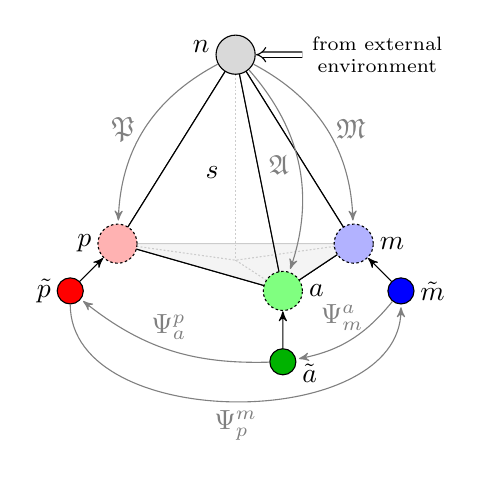
\begin{tikzpicture}[join=round,scale=3.0,node distance = -0.05]
		\tikzstyle{sign_comp}=[draw, circle,fill=white, scale=1.5];
		\tikzstyle{proto_comp}=[draw, circle,fill=white];
		
		\tikzstyle{label}=[align=center,fill=white,opacity=0.9,text opacity=1];
		\tikzstyle{coord_cine}=[dash pattern=on 0.7 off 0.7];
		\tikzstyle{ar_naming} = [->,>=stealth',shorten >=1pt,black!50];
		\tikzstyle{comp_tr} = [->,>=stealth'];		
		
		\filldraw[fill=white] (0.0,0.2) -- (0.5,1.0) -- (1.0,0.2) -- cycle;
		\filldraw[fill=black!20] (0.0,0.2) -- (0.7,0.0) -- (1.0,0.2) -- cycle;

		\draw[coord_cine] (0.5,1.0) -- (0.5,0.13);
		\draw[coord_cine] (0.0,0.2) -- (0.5,0.13);
		\draw[coord_cine] (0.7,0.0) -- (0.5,0.13);
		\draw[coord_cine] (1.0,0.2) -- (0.5,0.13);

		\filldraw[fill=white,fill opacity=0.8] (0.0,0.2) -- (0.5,1.0) -- (0.7,0.0) -- cycle;
		\filldraw[fill=white,fill opacity=0.8] (0.7,0.0) -- (0.5,1.0) -- (1.0,0.2) -- cycle;
				
		\node[sign_comp,fill = red!30,dash pattern=on 0.9 off 0.9] (s_p) at (0.0,0.2) {};
		\node[sign_comp,fill = blue!30,dash pattern=on 0.9 off 0.9] (s_m) at (1.0,0.2) {};
		\node[sign_comp,fill = gray!30] (s_n) at (0.5,1.0) {};
		\node[sign_comp,fill = green!50,dash pattern=on 0.9 off 0.9] (s_a) at (0.7,0.0) {};
		
		\node[left = of s_p] {$p$};
		\node[right = of s_m] {$m$};
		\node[yshift = 1mm, left = of s_n] {$n$};
		\node[right = of s_a] {$a$};
				
		\node[proto_comp,fill=red] (perc) at (-0.2,0.0) {};
		\node[proto_comp,fill=green!70!black] (bio) at (0.7,-0.3) {};
		\node[proto_comp,fill=blue] (func) at (1.2,0.0) {};

				
		\node[left = of perc] {$\tilde p$};
		\node[right = of func] {$\tilde m$};
		\node[yshift = -1.5mm, right = of bio] {$\tilde a$};
		
		\node[label] at ($(s_n)+(-0.1,-0.5)$) {$s$};
		
		\draw[ar_naming] (s_n) edge [bend right] node[left]{$\mathfrak P$}(s_p);
		\draw[ar_naming] (s_n) edge [bend left] node[right]{$\mathfrak M$}(s_m);
		\draw[ar_naming] (s_n) edge [bend left] node[left]{$\mathfrak A$}(s_a);
		
		\path[ar_naming] (perc) edge[out=-90, in=-90] node[below]{$\Psi_p^m$}(func);
		\draw[ar_naming] (func) edge [bend left=20] node[xshift = -1mm, above]{$\Psi_m^a$}(bio);
		\draw[ar_naming] (bio) edge [bend left=20] node[above]{$\Psi_a^p$}(perc);
		
		\draw[comp_tr] (perc) -- (s_p);
		\draw[comp_tr] (bio) -- (s_a);
		\draw[comp_tr] (func) -- (s_m);
		
		\node[align=center,font = \scriptsize] (cult) at (1.1,1.0){from external\\environment};
		
		\draw[-implies, >=stealth', double equal sign distance] (cult)-- (s_n);
	\end{tikzpicture}

\end{document}